\chapter{First-order model with application to Carlisle}

\section{Introduction}

The United Kingdom was subjected to numerous storms and severe floods throughout 2012, the wettest year for a century, resulting in lives lost and millions of pounds worth of damage. The UK was not alone, with similarly unusual weather events reported across the globe. As an example, in June 2013 an extreme flood event affected a substantial area of central Europe, resulting in 25 deaths and more than \euro{12bn} losses. This is not a new problem; the UK Environment Agency attributed two thirds of flooding during 2007 when a similarly wet season caused widespread disruption, to surface water and inadequacies in drainage \citep{Pitt2007}. In England alone over 5.2 million properties are known to be at risk of flooding, and annual investment must increase to more than a billion pounds per year just to maintain current levels of protection under the threat of climate change \citep{EnvironmentAgency2009a}. 

Attenuation of rainwater to reduce hydrograph peaks and alleviate surface water flooding is best achieved by sustainable drainage systems (SuDS) in urban areas. Comprehensive guidance is provided in the UK for the design and management of these by \citet{Woods-Ballard2007}. This stipulates that designs should consider and protect against overland flow originating off-site, and that the consequences of drainage blockage should be simulated. Such simulations are difficult to accomplish in practice, requiring high-resolution modelling of runoff source areas and all potential pathways to the site. Assessing the likely impacts of the proposed SuDS requires similarly high resolutions to represent the complex flow dynamics which might occur in wet ponds and infiltration basins, and to consider rates of sedimentation and maintenance requirements. Further complications are introduced by simulating hypothetical events affecting developments which have not and hopefully never will flood, meaning there is scarce data against which a parametric calibration might be performed. Where SuDS are in place, the residual risk remaining if the design storm is exceeded must be quantified to meet the recommendations of \citet{Pitt2007}.

Whilst the required high-resolution topographic data is increasingly available from airborne altimetric LiDAR, its wider application across large urban extents has largely been constrained by limitations in computational power and the performance of hydraulic modelling software. Research has understandably focussed in recent years on establishing how software models might be accelerated. Different techniques have been applied, such as dynamically adaptive grids, spatially-varying timesteps, and simplified approximations for the physics, with a particular emphasis on the latter. Dynamically adaptive grids retain the physical complexity but introduce new challenges in strictly maintaining both mass and momentum conservation, and will rarely increase the timestep if the most complex flow dynamics are represented at the highest resolutions \citep[e.g.][]{Liang2008,Kubatko2009}. A spatially-varying timestep complicates evaluation of inter-cell fluxes where cells have differing simulation times \citep{Sanders2011,Trahan2012}; furthermore, the efficiency gain does not always balance the workload associated with implementing a considerably more complex software structure. 

Elimination of terms from the shallow water equations (SWEs) gives rise to kinematic and diffusive wave approximations. These may allow faster computation at the expense of losing physical complexity, but compromise the predictive capabilities for flow velocity and by extension the time of inundation. Diffusive approximations are hindered at high resolutions by a strict timestep constraint, and kinematic approximations neglect potentially significant aspects of flow such as backwater effects \citep{Bates2000,Tsai2003,Hunter2005}. The topographic features of urban environments are characterised by narrow gaps between buildings and steep gradients; such conditions all have the potential to create transient flows, increase velocities, induce shocks, and cause backwater effects \citep{Testa2007,ElKadiAbderrezzak2011,Xia2011}. Comprehensive analysis of simplified approaches and the errors therein from numerical and pragmatic perspectives is given by \citet{Singh1996}, \citet{Hunter2007}, and \citet{Pender2010,Pender2013}. Simplified models are known to produce good results when calibrated against observed inundation data \citep[e.g.][]{Neal2009,Horritt2010} but parametric uncertainty and sensitivity is problematic for simulating hypothetical events \citep{Horritt2002,Yu2006,Fewtrell2008a}, as required for SuDS design.

Whilst transistor counts on central processing units (CPUs) continue to rise at rates comparable to Gordon Moore's observations, clock speed increases have stalled. Software developers must increasingly look to multi-core processing if they are to fully leverage the power of modern computers. Despite this a large number of commercial hydraulic modelling packages provide no such functionality, even though good weak and strong scaling can be accomplished \citep{Sanders2010,Kalyanapu2011,Saetra2012}. Heterogeneous computing and the advent of new methods (i.e. CUDA, OpenCL, DirectCompute) of interfacing with graphics processing units (GPUs) are even more promising: these devices are well-suited to performing the same calculation across large datasets, and are ideal for computational fluid dynamics (CFD). Much of the literature focuses on CUDA implementations which are constrained to operating on NVIDIA hardware \citep[e.g.][]{Kuo2011,Saetra2012}. Commercial software options for hydraulic modelling on GPU architectures are now available; a comparison can be found in \citet{Pender2013}, albeit limited to small domains which cannot fully capitalise on the parallel processing benefits \citep{Saetra2012}. The majority have yet to be released to the public, and all those the authors are aware of utilise CUDA and are hence limited to operating on NVIDIA hardware. Herein we describe how OpenCL allows a single codebase to be used for parallel computation with either CPU or GPU devices available any of the mainstream vendors. 

The work of \citet{Ozdemir2013} explicitly considers the benefits of high-resolution modelling for SuDS design, emphasising that increased topographic detail improves results beyond the range of parametric calibration. Simulation run-times and instabilities are recognised therein as barriers to wider application, but nonetheless best practice guidance encourages the use of detailed hydraulic modelling for long-term storage design \citep{Woods-Ballard2007}. Herein, we contribute towards resolving both of these problems. We describe how a robust finite-volume Godunov-type scheme is implemented for new software, and applied to simulate flow dynamics during a flood at the whole-city scale with a high-resolution grid. 

\section{Methodology}

We first consider a numerical scheme appropriate for use in urban flood modelling. As a minimum the scheme must appropriately address complex flow dynamics for transient flow conditions where shocks may be present. It must also be able to handle cell wetting and drying, depict a lake at rest even with uneven bed topography, and preserve depth positivity. We then transpose the approach to a computational framework suitable for parallel execution with various types of processing device. 

\subsection{Finite-volume Godunov-type scheme}

It is generally true that the vertical scale of the fluid flows is much smaller than the horizontal for flood events. It is therefore appropriate to approximate the flood wave dynamics with the SWEs derived by depth integrating the Reynolds-averaged Navier-Stokes equation. This hyperbolic system of conservation laws accounts for both mass and momentum conservation, and is presented in vector notation as

\begin{equation}
	\label{SWE}
	\frac{\partial\textbf{U}}{\partial t} +
	\frac{\partial\textbf{F}}{\partial x} +
	\frac{\partial\textbf{G}}{\partial y} =
	\textbf{S} ,
\end{equation}

where t is the simulation time, \(x\) and \(y\) refer to the Cartesian coordinate space, \(\textbf{U}\) is the vector of flow variables, \(\textbf{F}\) and \(\textbf{G}\) are fluxes in the two respective Cartesian dimensions, and \(\textbf{S}\) is a source term vector through which inflow and losses may be accounted for. The equation is solved within a regular two-dimensional Cartesian domain, for which the vector terms of equation \eqref{SWETerms} are as described in \citet{Liang2009b}, 
 
\begin{equation}
	\label{SWETerms}
	\begin{alignedat}{4}
		&\textbf U && = \left[ \begin{array}{c}
			\eta \\
			uh \\
			vh
		\end{array} \right] , ~ &&
		\textbf F &&  = \left[ \begin{array}{c}
			hu \\
			hu^2 + \frac{1}{2}(g\eta^2 - 2\eta z_b) \\
			huv
		\end{array} \right] ,\\
		&\textbf G && = \left[ \begin{array}{c}
			hv \\
			hvu \\
			hv^2 + \frac{1}{2}(g\eta^2 - 2\eta z_b) \\
		\end{array} \right] , ~ &&
		\textbf S && = \left[ \begin{array}{c}
			0 \\
			-\frac{\tau_bx}{\rho} - g\eta \frac{\partial z_b}{\partial x} \\
			-\frac{\tau_by}{\rho} - g\eta \frac{\partial z_b}{\partial y} \\
		\end{array} \right] .
	\end{alignedat}
\end{equation}

Here, \(\eta\) and \(z_{b}\) are the free surface level and bed elevation for the underlying topography respectively; \(h = \eta - z_{b}\) gives the total water depth; for the two Cartesian directions, \(u\) and \(v\) are depth-averaged velocities, \(qx (=uh)\) and \(qy (=vh)\) are volumetric discharge per unit width, \(\tau_{bx}\) and \(\tau_{by}\) are bed shear stresses, \(\partial{z_{b}} / \partial{x}\) and \(\partial{z_{b}} / \partial{y}\) define the bed slopes; \(g\) is acceleration due to gravity, \(\rho\) is the water density; and \(q_{0}\) denotes a source or sink for mass (e.g. rainfall, drainage outfall, etc.).

A Godunov-type scheme is used to solve equation \eqref{SWE} and ensure complex flow dynamics are represented (e.g. hydraulic jump transitions). Local solutions to the Riemann problem across each cell interface are hence used to update each cell state with the time-marching formula,

\begin{equation}
	\label{GodunovUpdate}
	\begin{alignedat}{2}
	\textbf{U}^{t+\Delta t} = \textbf{U}^t & - \frac{\Delta t}{\Delta x}(\textbf{F}^+ - \textbf{F}^-) 
					     &  - \frac{\Delta t}{\Delta y}(\textbf{G}^+ - \textbf{G}^-) + \Delta t \textbf{S} , 
	\end{alignedat}
\end{equation}

where \(\textbf{F}^-\), \(\textbf{F}^+\), \(\textbf{G}^-\), \(\textbf{G}^+\) are fluxes through a cell's western, eastern, southern and northern interfaces respectively. As a result of the explicit numerical scheme, the timestep \(\Delta{t}\) is constrained as per the conditions described by \citet{Courant1967},

--SNIP--

where \(0 < C \le 1\). Depth positivity is preserved through reconstruction of the interface state pair before computing fluxes \citep{Liang2010a}, for which a piecewise distribution of flow information is assumed, allowing a single bed elevation and current conditions to be identified as

\begin{equation}
	\label{Reconstruction1}
		\hat{h}^L = \hat{\eta}^{L} - \hat{z_{b}}^{L}, \hfill
		\hat{u}^L = \hat{q_x}^{L} / \hat{h}^{L}, \hfill
		\hat{v}^L = \hat{q_y}^{L} / \hat{h}^{L}, \hfill and \hfill
		z_b = max( \hat{z_b}^{L} , \hat{z_{b}}^{R} ) , \hfill
\end{equation}

where superscript \(L\) and \(R\) indicate sides of the interface, and \(\hat{}\) indicates the values before reconstruction. From here the new discharge per unit width and free-surface levels are deduced,

\begin{equation}
	\label{Reconstruction2}
		h^L = max( 0, \hat{\eta}^{L} - z_{b} ), \hfill
		\eta^L = h^L + z_b, \hfill
		q_x^L = \hat{u}^L\hat{h}^L, \hfill and \hfill
		q_y^L = \hat{v}^L\hat{h}^L . \hfill
\end{equation}

Finally, a local bed modification is applied to ensure the free-surface level does not fall below the bed elevation, a condition which would otherwise give rise to spurious fluxes,

\begin{equation}
	\label{Reconstruction3}
		\Delta{z} = max( 0, z_{b} - \hat{\eta}^{L} ), \hfill
		z_b \gets z_b - \Delta{z}, \hfill and \hfill
		\eta^L \gets \eta^L - \Delta{z} . \hfill
\end{equation}

The process is similarly repeated for the right side of the cell interface. These reconstructed state values for both sides of a cell interface define local Riemann problems, solved by the HLLC approximate solver to obtain fluxes, thereby accounting for physical features of discontinuities including contact and shear waves \citep{Toro1994} and shown to perform well with differing flow conditions \citep{Erduran2002}. The bed slope component of the source term vector in \eqref{SWETerms} is approximated through a central differencing approach. 

The friction source terms are solved independently of the main scheme using a point-implicit approach obtained through Taylor expansion, as proposed by \citet{Liang2010a}. 

\subsection{Software framework for CPU and GPU computation}

\begin{figure*}[tpb]
\centering
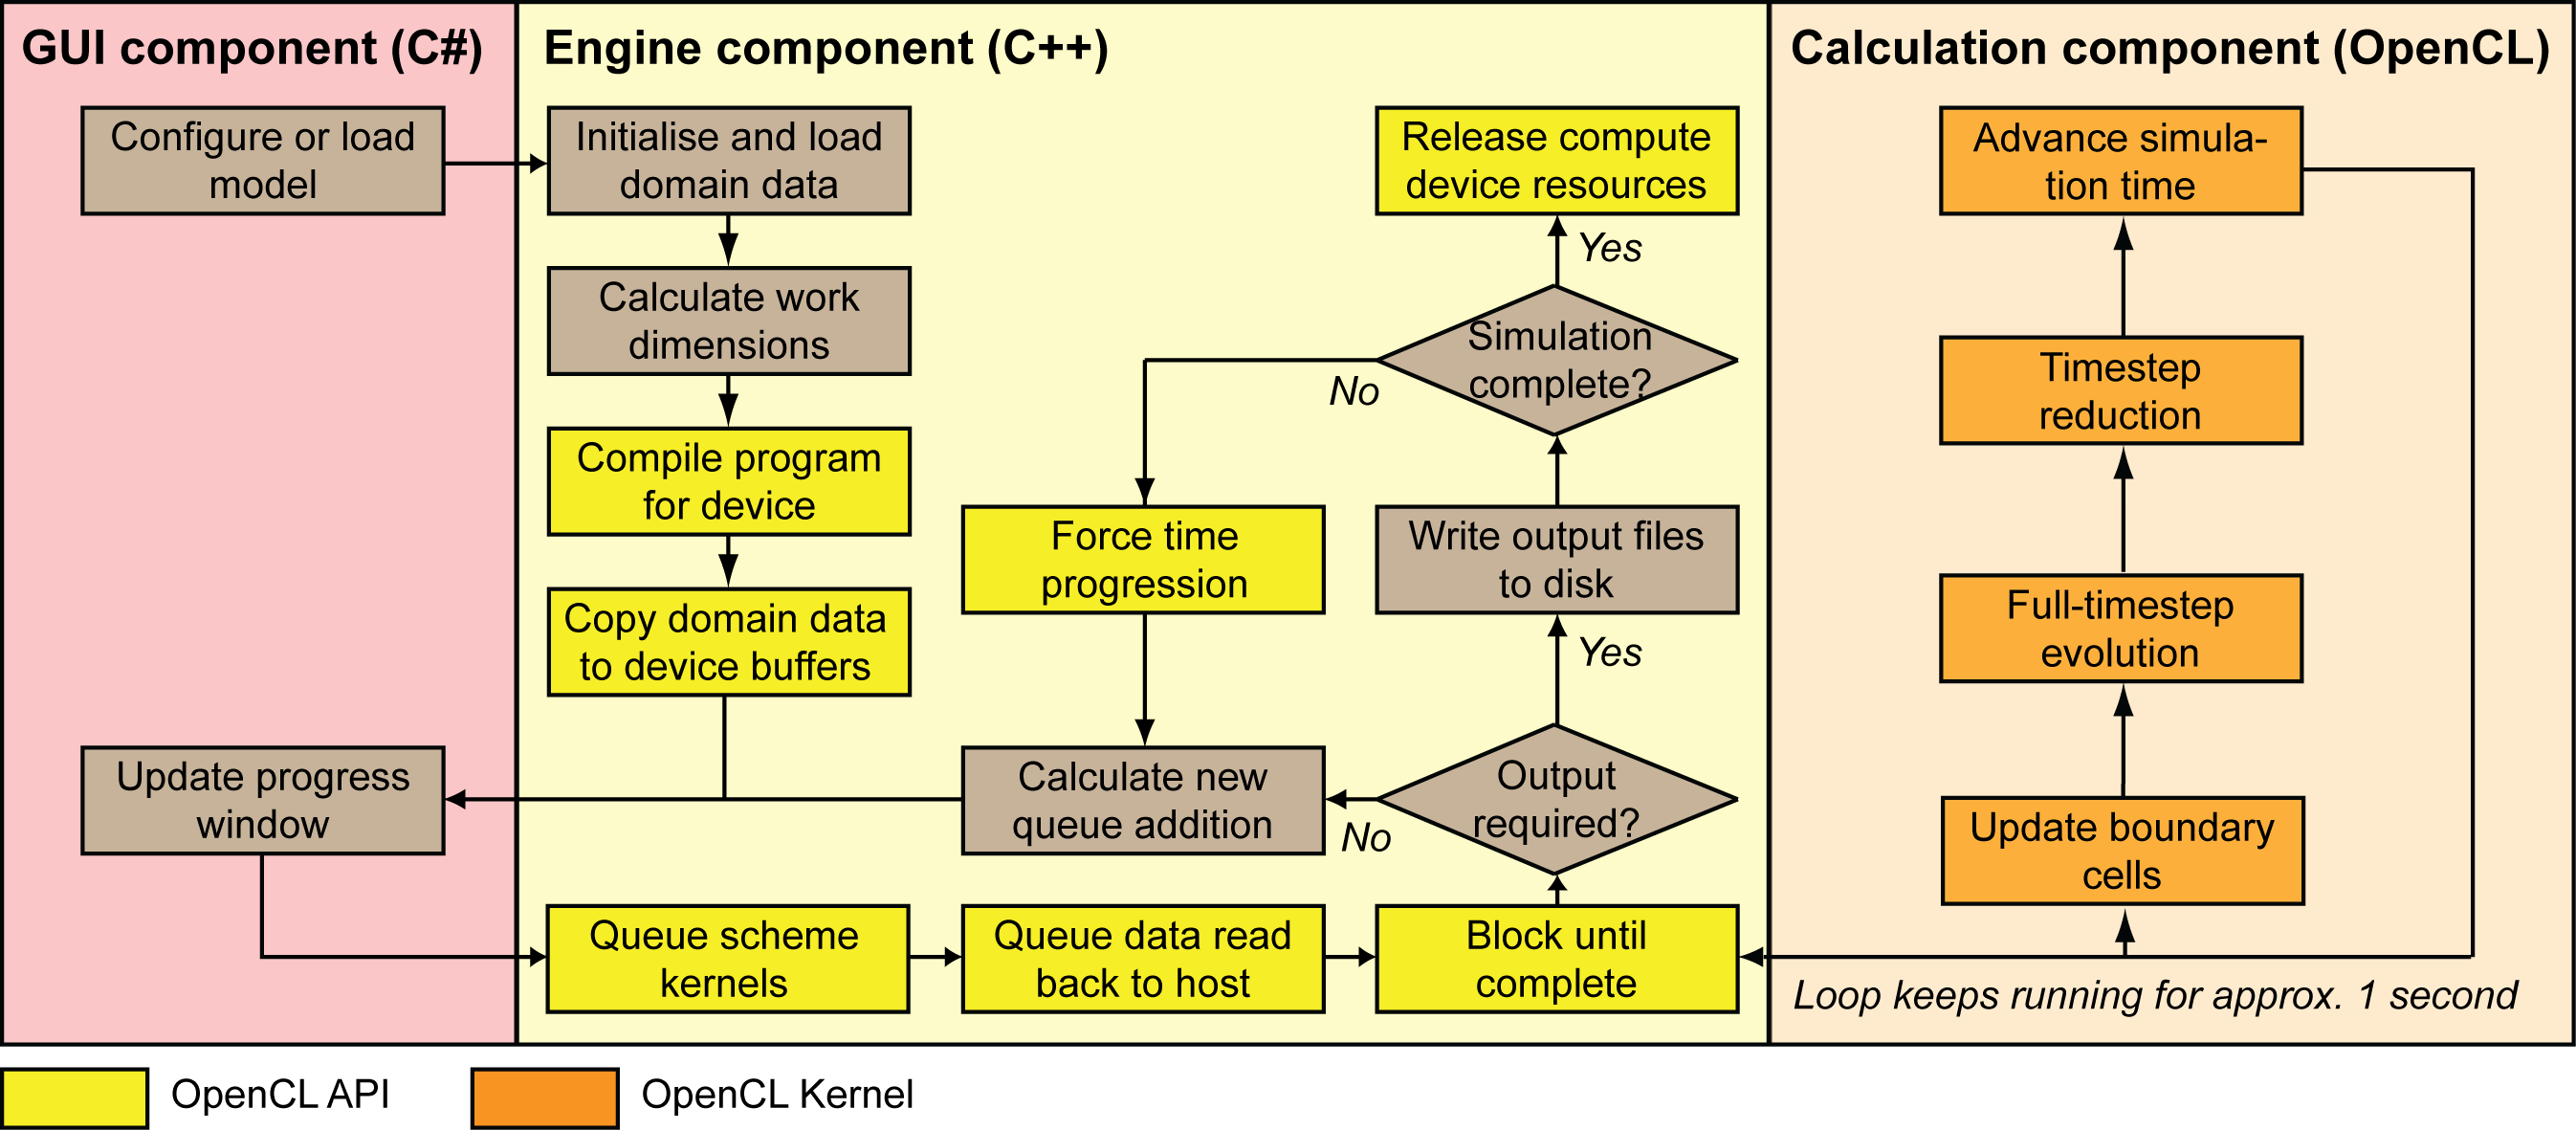
\includegraphics[width=1.0\textwidth]{carlisle-figures/Figure1.png}
\caption{Graphical representation of the software structure and main processes.}
\label{SoftwareProcesses}
\end{figure*}

Achieving high levels of performance for GPU devices requires careful consideration of the program structure and resource consumption in order to fully harness different processor architectures. Optimal levels of performance are achieved if a processing device is consistently occupied with work, allowing data transfers from global device memory (RAM) to processing unit specific registers to occur asynchronously in the background and the significant latency associated therewith to be masked. The underlying hardware manages the synchronisation of work across the resources available through the similar concepts of warps (NVIDIA) and wavefronts (AMD). Processing devices may only access data held within their own respective memories, thus duplicate copies of the domain data are required to reside in both GPU and CPU memory. Transferring data over the main system bus is an expensive operation, which should be as infrequent as possible.

The domain is considered as a single Cartesian grid with data stored in linear memory structures. 64-bit floating-point computation requires 48 bytes per cell including friction coefficients, which allowing for further constraints imposed by the device, permits up to 50 million cells per domain with GPU devices currently available before the maximum OpenCL buffer size is likely to be exceeded. Computation of larger domains within a single device would remain possible if cell data was split across multiple memory buffers. The numerical scheme is mapped to a series of small discrete programs (i.e. kernels in OpenCL terminology) which may run sequentially for multiple iterations before any data needs to be transferred back to the CPU. This allows efficient execution, with data transferred approximately every second to update the user on simulation progress, and write output files to disk if required. As a whole the software is structured as three discrete application elements of differing programming languages; a graphical representation of this model is shown in Figure \ref{SoftwareProcesses}: the graphical user interface is responsible only for allowing the user to configure a model, and providing status updates; the engine component is responsible for loading the required data, identifying suitable devices to be used in computation, coordinating the work required for the simulation, and writing output files at a user-defined interval. The calculation component is wholly parallelised, but to alleviate potential inefficiency resulting from the latency associated with host-bus transfers to GPU devices, several iterations of the numerical scheme can be scheduled to run independently before the engine component becomes aware of progress. This loop in the calculation component typically runs for approximately one second after the blocking command is issued in the engine component, after which it is assumed the user should be updated on simulation progress; the number of iterations is therefore a function of the size of the domain.

The scheme is effectively programmed as a stencil operation, for which the kernel is executed across every cell in the domain, but each requires data from its four immediate neighbours. Two memory buffers hold transient cell data as four-element vectors (consisting free-surface level, maximum level, and unit-width discharge in the x- and y-directions). The buffers are swapped each time the scheme kernels are queued (i.e. the target memory becomes the source memory for the next iteration). The outer-most layer of cells is exempt from the full-timestep evolution kernel, allowing these cells to provide reflective or transmissive boundary conditions. Only a first-order solution is used herein; a GPU implementation of the second-order accurate MUSCL-Hancock scheme within the same framework, and more in-depth discussion of the challenges for achieving computational efficiency can be found in \citet{Smith2013}. Boundary conditions are imposed directly at ghost cells exempt from processing at the edge of the computational domain, as in \citet{Liang2010a}.

\begin{figure*}[tpb]
\centering
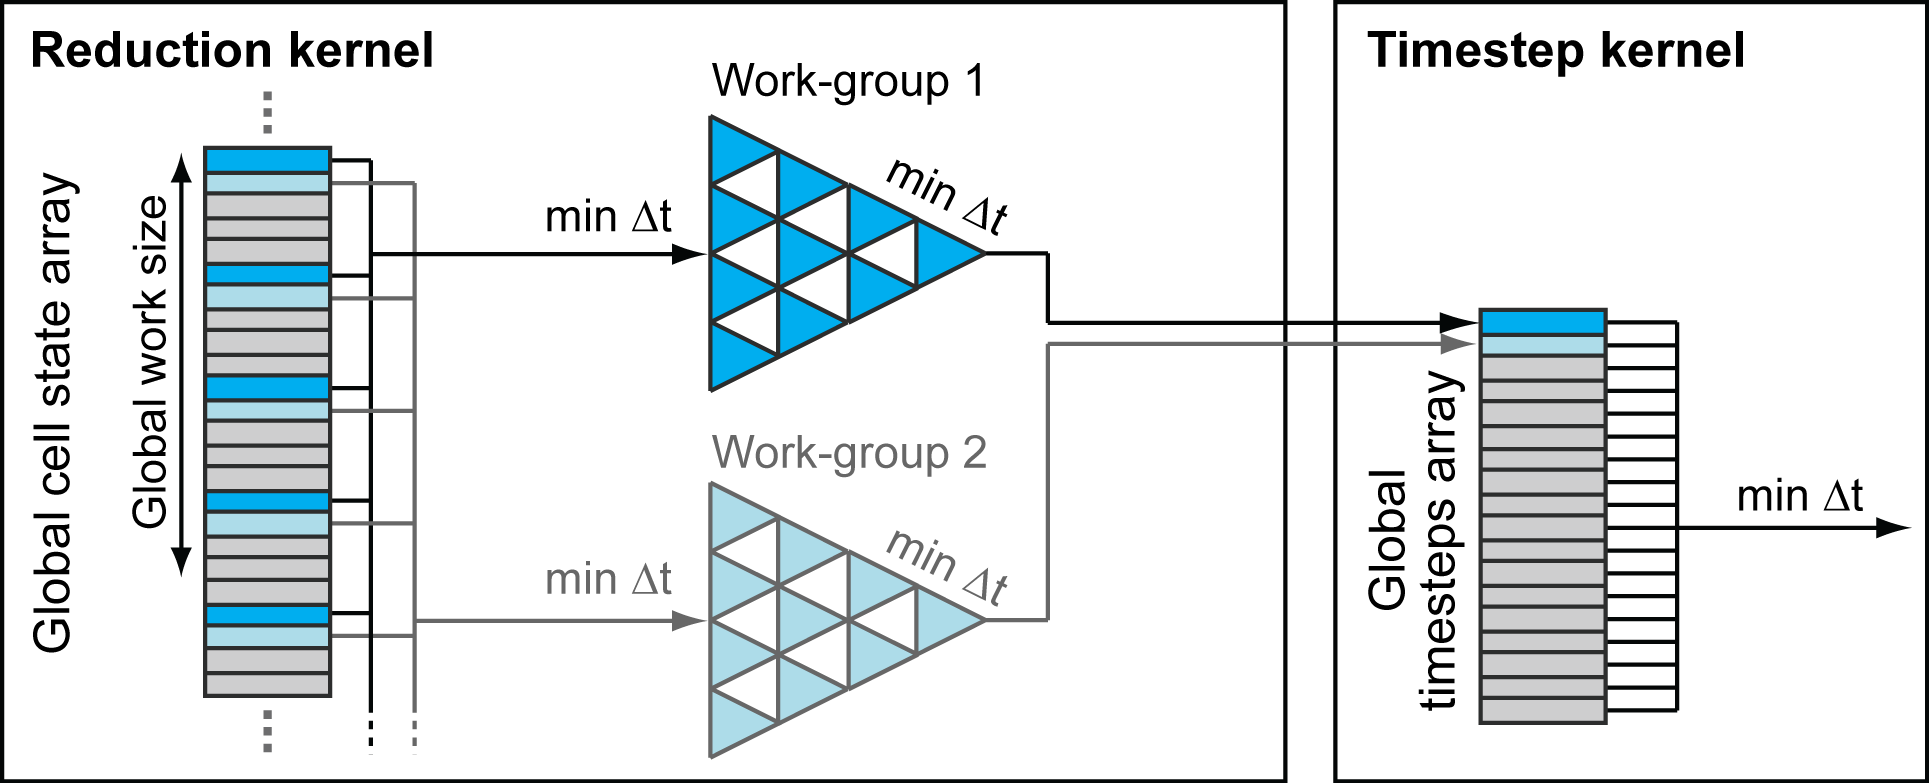
\includegraphics[width=0.8\textwidth]{carlisle-figures/Figure2.png}
\caption{Illustration of the reduction two-stage reduction process used to identify the timestep.}
\label{ReductionDiagram}
\end{figure*}

Implementation of the timestep constraint given in equation (4) requires identification of the greatest velocity present in the domain after each iteration of the numerical scheme, to create a variable timestep thus ensuring the stability of the numerical scheme. A two-stage reduction (i.e. identifying the minimum permissible timestep from a large number of cells) process adopted herein allows a large enough quantity of work per compute unit to mask memory latency through smaller but more intensive work dimensions. Domain cells are sampled with a regular stride until the end of the cell array is reached, then successive binary comparisons are carried out in multiple iterations until other threads within the group have been retired and a single value remains. This is carried forward to a new much smaller array of potential timesteps, which is examined finally when the simulation time is advanced. The process is illustrated in Figure \ref{ReductionDiagram}. The timestep is constrained to 0.1 seconds for the first minute of the simulation while the first water enters the domain. 

A perhaps unusual approach is adopted with OpenCL, allowing the code for the numerical scheme to be dynamically generated and complied at the point of use by the underlying system drivers with an instruction set specific to the hardware available. This allows code which is not required or disabled (e.g. second-order accuracy, friction effects) to be omitted altogether, and constants such as the domain dimensions to be stored within the program binary. The compiler is instructed to adhere to all of the appropriate IEEE standards for floating-point computation, hence standards-compliant CPUs and GPUs alike should produce identical results.

\section{Results and discussion}

Snipped.

\section{Conclusions}

The software presented herein is successfully applied to reproduce the flooding which occurred in Carlisle during 2005. The same approach can easily be used to model surface water flooding, and to assess the impact of potential SuDS designs. Further improvement in the accuracy of the simulations would be difficult to assess given the error inherently present in the validation datasets. GPUs have allowed high-resolution simulations to be carried out with a robust and physically accurate numerical approach for hydrodynamic modelling in a matter of hours rather than days. The techniques adopted capitalise on parallel processing with the flexibility to operate across a wide range of devices currently available from mainstream hardware vendors; software developers for hydrodynamic models must respond to the stagnation of processor clock speeds and harness parallelism to take advantage of the most recent increases in computing power. 

High-resolution modelling has accurately represented and constrained the complex flow dynamics to within the river channel, and as a consequence we have observed decreasing sensitivity for the floodplain with higher resolutions, resulting in extremely low sensitivity at 2m resolution. This demonstrates the importance of accurately representing the topography within hydrodynamic models, but overland flow velocities might be higher during surface water flooding. Further work is required to corroborate and explore parametric sensitivity. Different types of urban flood events should be simulated with high spatial resolutions and parametric sensitivity examined. The authors also intend to extend the software to use multiple GPUs for a single simulation, and will provide details in a forthcoming publication.

